\chapter{Special Relativity: Reference Frames, Light, and Spacetime}

This quarter returns to classical physics, but now at its relativistic end. We have learned the general structure of Newtonian mechanics, and we have had a first pass through quantum mechanics, but light has not yet really entered the story. That is why special relativity comes first: it is the gateway to classical field theory, and in particular to electromagnetism. These notes follow Leonard Susskind's first lecture in the 2012 spring \emph{Theoretical Minimum} course on special relativity, with the lecture's board rhythm preserved and with supporting frame evidence curated through LazyingArt LLC and Video2Book.

\section{Why Begin Again?}

Susskind opens by asking the room whether special relativity should be reviewed at all. Almost everyone has seen it before, and yet the room votes to go through it. That choice matters. He is not reviewing reluctantly; he is deliberately rebuilding the subject from the beginning so that each step will later have a visible reason behind it. We are not to start from the Lorentz transformation as a fact to be memorized. We are to see why the old picture breaks, and what replaces it.

So he backs up one step before relativity itself and asks for the notion of a reference frame.

\paragraph{Reference frames.}
A reference frame begins with spatial coordinates \(x,y,z\), together with an origin and an orientation. If we want to think concretely, we imagine space filled with a lattice of meter sticks. Every point can then be specified as so many meters to the left or right, up or down, in or out, from the origin. To say when something happens, we add a time coordinate \(t\), which means we imagine a synchronized set of clocks spread throughout space.

\begin{definition}
A reference frame is a coordinate system for space and time, concretely realized as a lattice of meter sticks together with synchronized clocks. An inertial reference frame is one in which force-free particles move with uniform velocity.
\end{definition}

Two observers in relative motion assign different coordinates to the same event. They certainly disagree about position. If I carry my own coordinates with me, then in my system my nose may always sit at some fixed \(x'\), while in your frame that same nose moves and its coordinate changes with time. In pre-relativistic physics one also assumed that time caused no such difficulty: our watches, once synchronized, remained in agreement, and one wrote simply
\begin{equation}
t'=t.
\end{equation}
That was the Newtonian assumption hiding inside the old kinematics.

\paragraph{Relativity before Einstein.}
The principle of relativity did not begin with Einstein. In Newtonian mechanics one already says that the laws of physics are the same in all inertial reference frames. The lecture hall version of this is the railroad train: if we are inside a train moving uniformly and the windows are sealed, the laws of juggling are the same as at rest. Balls go up and down as before. Forces and inertia behave as before. One cannot detect uniform motion from within the inertial frame itself.

What Einstein adds is not the principle of relativity in the vague sense, but one more law of physics:
\begin{equation}
\text{light moves with speed } c.
\end{equation}
Once we combine that law with the older principle of relativity, we are driven into a puzzle. If the laws of physics are the same in every inertial frame, and the speed of light is one of those laws, then every inertial observer must assign the same speed \(c\) to light. That is the tension the lecture now makes precise.

\section{The First Puzzle: Light and the Failure of the Galilean Rule}

Susskind now becomes intentionally pedantic. He throws away two spatial dimensions and keeps only one. We draw an \(x\)-axis and a \(t\)-axis. That is enough to see the problem.

\begin{figure}
\centering

\includegraphics[width=0.72\textwidth]{lecture_01_figure_02.png}
\caption{Spacetime axes as the light trajectory is introduced. Only the beginning \(x=\) is visible on the board; the completed equation \(x=ct\) follows from the transcript.}
\end{figure}

In the stationary frame, a light ray emitted from the origin has trajectory
\begin{equation}
x=ct.
\end{equation}
On the spacetime diagram this is a straight line.

\begin{figure}
\centering
\begin{tikzpicture}[scale=0.95]
\draw[->] (0,0) -- (5.8,0) node[right] {$x$};
\draw[->] (0,0) -- (0,4.8) node[above] {$t$};
\draw[thick] (0,0) -- (5.0,3.0);
\node at (4.35,2.45) {$x=ct$};
\end{tikzpicture}
\caption{A clean redraw of the first spacetime picture. The slope is fixed by the speed \(c\).}
\end{figure}

Now add a second observer moving uniformly to the right. In the unprimed coordinates that observer's world line is
\begin{equation}
x=vt.
\end{equation}
The moving observer, of course, does not call that line \(x=vt\). He calls it his own location:
\begin{equation}
x'=0.
\end{equation}

\begin{figure}
\centering

\includegraphics[width=0.72\textwidth]{lecture_01_figure_03.png}
\caption{The moving observer's world line \(x=vt\), drawn against the light trajectory. The unlabeled green line is identified from the surrounding lecture context as the light ray.}
\end{figure}

\begin{figure}
\centering
\begin{tikzpicture}[scale=0.95]
\draw[->] (0,0) -- (5.8,0) node[right] {$x$};
\draw[->] (0,0) -- (0,5.2) node[above] {$t$};
\draw[thick] (0,0) -- (5.0,3.0);
\draw[thick] (0,0) -- (2.35,5.0);
\node at (4.35,2.55) {$x=ct$};
\node at (2.55,4.6) {$x=vt$};
\node at (1.55,3.25) {$x'=0$};
\end{tikzpicture}
\caption{Light and an ordinary world line on the same \(x\)-\(t\) plane. Since \(v<c\), the material world line is steeper than the light ray.}
\end{figure}

If we now use the old Newtonian rule, the coordinates are related by
\begin{equation}
x'=x-vt,\qquad t'=t.
\end{equation}
Apply this to the light ray. Along \(x=ct\),
\begin{equation}
x'=ct-vt=(c-v)t=(c-v)t'.
\end{equation}
So in the moving frame the light ray seems to move with speed \(c-v\), not \(c\). For a left-moving light ray \(x=-ct\), the same rule gives
\begin{equation}
x'=-(c+v)t=-(c+v)t'.
\end{equation}
One direction comes out too slow, the other too fast. That is bad. Something is wrong.

The lecture insists on the diagnosis: if Einstein is right about light, then something is wrong with the transformation law between your coordinates and mine. The old rule is the thing to put on trial.

\subsection{Question \& Answer}

If the laws of physics are the same in every inertial frame, why does the naive coordinate change make light move at different speeds?

Because the naive coordinate change smuggles in a Newtonian assumption that has not been earned. The spatial shift \(x'=x-vt\) is not yet the deepest problem. The dangerous part is
\[
t'=t.
\]
That equation assumes that simultaneity is the same in every inertial frame. Special relativity begins when we stop taking that for granted.

\section{Einstein Synchronization and the Relativity of Simultaneity}

Before changing formulas, Susskind changes the question. What do we actually mean when we say that distant clocks are synchronized?

Take two clocks, one at the left and one at the right, and place a third observer at the midpoint. The left and right clocks are first checked to be equally distant from the midpoint using meter sticks. Then the two end clocks agree to send flashes of light when each reads noon. If the flashes arrive together at the midpoint, the clocks are synchronized. That is Einstein's operational definition.

This is already a significant shift. Simultaneity is no longer an undefined background notion. It is something established by a physical procedure involving light, distance, and clocks.

Now imagine that those clocks are synchronized in the stationary frame. A moving observer passes the midpoint just as the flashes are emitted. The flashes do not reach the midpoint instantly; by the time they arrive, the moving observer has moved off center. One flash reaches him before the other. He therefore concludes that the stationary clocks were not synchronized in his frame.

So the meaning of simultaneity depends on the frame. In the stationary frame, events that are simultaneous lie on horizontal lines,
\begin{equation}
t=\text{const}.
\end{equation}
In the moving frame, the corresponding lines of simultaneity will not be horizontal.

\subsection{Question \& Answer}

What does it actually mean to say that distant clocks are synchronized?

It means that a synchronization procedure has been carried out: equally distant clocks send light signals toward a midpoint, and those signals arrive together. That is the content of the statement. Once the speed of light is taken to be the same in every inertial frame, different observers need not agree on the outcome of that procedure. Thus simultaneity is not absolute; it is frame-dependent.

\section{Building the Moving Geometry in Spacetime}

Having diagnosed the problem, the lecture returns to the diagram. The first rule is methodological as much as physical: whenever we encounter a relativity problem, draw a picture. And before drawing anything else, draw the light rays.

At this stage Susskind switches to relativistic units by setting \(c=1\). If time is measured in seconds and length in light-seconds, then light travels one unit of length in one unit of time, and the light rays lie at \(45^\circ\):
\begin{equation}
x=\pm t.
\end{equation}

We then redraw the moving observer and a family of parallel world lines attached to the moving frame. The board labels the first two directly; the third is reconstructed cautiously from the lecture's spoken sequence.

\begin{figure}
\centering

\includegraphics[width=0.78\textwidth]{lecture_01_figure_05.png}
\caption{Parallel moving world lines against the light rays. The board directly shows \(x=vt\), \(x'=0\), and \(x=vt+1\); the next line is completed from the lecture as \(x=vt+2\).}
\end{figure}

\begin{figure}
\centering
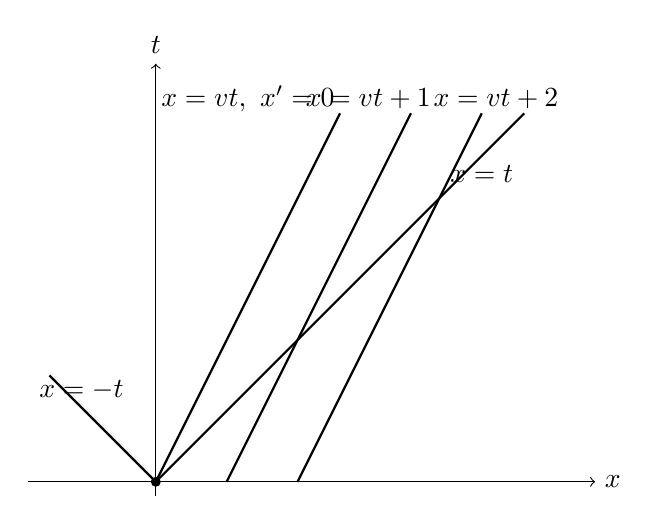
\begin{tikzpicture}[scale=0.9]
\draw[->] (-1.8,0) -- (6.2,0) node[right] {$x$};
\draw[->] (0,-0.2) -- (0,5.9) node[above] {$t$};
\fill (0,0) circle (2pt);
\draw[thick] (0,0) -- (5.2,5.2);
\draw[thick] (0,0) -- (-1.5,1.5);
\draw[thick] (0,0) -- (2.6,5.2);
\draw[thick] (1.0,0) -- (3.6,5.2);
\draw[thick] (2.0,0) -- (4.6,5.2);
\node at (1.3,5.4) {$x=vt,\ x'=0$};
\node at (3.0,5.4) {$x=vt+1$};
\node at (4.8,5.4) {$x=vt+2$};
\node at (4.6,4.35) {$x=t$};
\node at (-1.05,1.3) {$x=-t$};
\end{tikzpicture}
\caption{A clean redraw of the board geometry in units with \(c=1\). Light rays are drawn first; the moving family comes afterward.}
\end{figure}

Now comes the geometric heart of the lecture. We place three observers in the moving frame: Fred on \(x=vt\), Mary on \(x=vt+1\), and Seymour on \(x=vt+2\). The origin is the event at which the stationary and moving observers agree to call the time zero. Fred sends a light signal from the origin to Mary. Seymour must send his own light signal so that it reaches Mary at the same instant. That requirement defines which event on Seymour's world line is simultaneous with the origin in the moving frame.

\begin{figure}
\centering
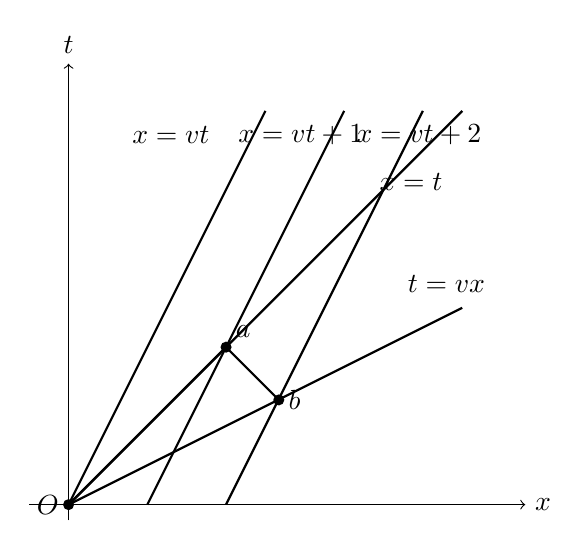
\begin{tikzpicture}[scale=1.0]
\draw[->] (-0.5,0) -- (5.8,0) node[right] {$x$};
\draw[->] (0,-0.2) -- (0,5.6) node[above] {$t$};
\draw[thick] (0,0) -- (5.0,5.0);
\draw[thick] (0,0) -- (2.5,5.0);
\draw[thick] (1.0,0) -- (3.5,5.0);
\draw[thick] (2.0,0) -- (4.5,5.0);
\fill (0,0) circle (2pt);
\fill (2,2) circle (2pt);
\fill (2.67,1.33) circle (2pt);
\draw[thick] (0,0) -- (2,2);
\draw[thick] (2.67,1.33) -- (2,2);
\draw[thick] (0,0) -- (5.0,2.5);
\node[left] at (0,0) {$O$};
\node[above right] at (2,2) {$a$};
\node[right] at (2.67,1.33) {$b$};
\node at (1.3,4.7) {$x=vt$};
\node at (2.95,4.7) {$x=vt+1$};
\node at (4.45,4.7) {$x=vt+2$};
\node at (4.35,4.1) {$x=t$};
\node at (4.8,2.8) {$t=vx$};
\end{tikzpicture}
\caption{The Fred--Mary--Seymour construction. Point \(a\) is where Fred's light reaches Mary; point \(b\) is the event on Seymour's world line from which a light signal reaches Mary at the same instant. The line through \(O\) and \(b\) is the moving simultaneity line \(t'=0\).}
\end{figure}

Let us work it out. Point \(a\) lies at the intersection of the right-moving light ray
\begin{equation}
x=t
\end{equation}
and Mary's world line
\begin{equation}
x=vt+1.
\end{equation}
Substituting \(x=t\) into the second equation gives
\begin{equation}
t=vt+1,
\end{equation}
so
\begin{equation}
t_a=\frac{1}{1-v}.
\end{equation}
Since \(a\) lies on \(x=t\), we immediately get
\begin{equation}
x_a=\frac{1}{1-v}.
\end{equation}

Now take the light ray from \(a\) downward to the right, or equivalently upward to the left. Any such \(45^\circ\) line in these units satisfies
\begin{equation}
x+t=\text{const}.
\end{equation}
Evaluating that constant at \(a\), we find
\begin{equation}
x+t=\frac{2}{1-v}
\end{equation}
all along the line \(ab\). The transcript stumbles slightly at this point, but the geometry and the algebra fix this constant unambiguously.

Point \(b\) lies on Seymour's world line, so it also satisfies
\begin{equation}
x=vt+2,
\end{equation}
or equivalently
\begin{equation}
x-vt=2.
\end{equation}
Thus \(b\) is found by solving the simultaneous equations
\begin{align}
x+t &= \frac{2}{1-v}, \\
x-vt &= 2.
\end{align}
Subtracting the second equation from the first eliminates \(x\):
\begin{equation}
(1+v)t=\frac{2}{1-v}-2=\frac{2v}{1-v}.
\end{equation}
Therefore
\begin{equation}
t_B=\frac{2v}{1-v^2}.
\end{equation}
Substituting back gives
\begin{equation}
x_B=\frac{2}{1-v^2}.
\end{equation}

Why did we go through all of that? Because the entire moving line of simultaneity through the origin must pass through \(b\). Its slope is therefore
\begin{equation}
\frac{t_B}{x_B}=v.
\end{equation}
Hence the line itself is
\begin{equation}
t=vx.
\end{equation}
This is the line \(t'=0\).

That is the geometric breakthrough. We now know two vanishing conditions:
\begin{equation}
x'=0 \quad \Longleftrightarrow \quad x=vt,
\end{equation}
and
\begin{equation}
t'=0 \quad \Longleftrightarrow \quad t=vx.
\end{equation}
From here the algebra can begin in earnest.

\section{From Geometry to Algebra: Deriving the Lorentz Transformation}

The lecture now resets the board. The left side still carries the worked geometry, but the right side begins anew with the most general transformation consistent with what we have learned.

\begin{figure}
\centering

\includegraphics[width=0.82\textwidth]{lecture_01_figure_06.png}
\caption{The derivation resets from the detailed spacetime construction to the general ansatz. The left board still records the previous worked example; the right board isolates the transformation law.}
\end{figure}

What more do we know? We know that \(x'=0\) whenever \(x=vt\). That means \(x'\) must contain the factor \(x-vt\). Up to an unknown velocity-dependent scale factor,
\begin{equation}
x'=(x-vt)f(v).
\end{equation}
Likewise, because \(t'=0\) whenever \(t=vx\), we must have
\begin{equation}
t'=(t-vx)g(v).
\end{equation}
At this point \(f\) and \(g\) are unknown. By symmetry one expects them to depend only on the relative speed, but their actual form has not yet been determined.

Now we use some physics. In the unprimed frame, a right-moving light ray obeys
\begin{equation}
x=t.
\end{equation}
Einstein's postulate says that in the moving frame it must also move with speed \(1\), so along that same ray we must have
\begin{equation}
x'=t'.
\end{equation}
But when \(x=t\),
\begin{align}
x'&=(1-v)x\,f(v),\\
t'&=(1-v)x\,g(v).
\end{align}
These can agree for all points on the light ray only if
\begin{equation}
f(v)=g(v).
\end{equation}
So both transformations carry the same factor:
\begin{align}
x'&=(x-vt)f(v),\\
t'&=(t-vx)f(v).
\end{align}

What more do we want to know? We want to know what \(f(v)\) is. Here Susskind appeals to reciprocity. If the primed frame moves with velocity \(v\) relative to the unprimed frame, then the unprimed frame moves with velocity \(-v\) relative to the primed frame. Therefore the inverse transformation must have the same form:
\begin{align}
x&=(x'+vt')f(v),\\
t&=(t'+vx')f(v).
\end{align}
The lecture transcript becomes rough around the inverse formulas, but by symmetry this is the clean statement.

Now substitute the direct transformation into the inverse expression for \(x\):
\begin{align}
x&=\Bigl[(x-vt)f(v)+v(t-vx)f(v)\Bigr]f(v)\\
 &=\bigl[x-vt+vt-v^2x\bigr]f(v)^2\\
 &=x(1-v^2)f(v)^2.
\end{align}
For this to make sense at all, the right-hand side must reduce to \(x\). Hence
\begin{equation}
(1-v^2)f(v)^2=1.
\end{equation}
Therefore
\begin{equation}
f(v)=\frac{1}{\sqrt{1-v^2}}.
\end{equation}
There is also a negative root, but continuity at \(v=0\) fixes the physical choice. When the relative velocity vanishes, we want
\[
x'=x,\qquad t'=t,
\]
not a reflection \(x'=-x\).

So in units with \(c=1\), the Lorentz transformation is
\begin{align}
x'&=\frac{x-vt}{\sqrt{1-v^2}},\\
t'&=\frac{t-vx}{\sqrt{1-v^2}}.
\end{align}
These are the equations that replace the old Newtonian rule. They have been constructed so that the light rays remain at \(45^\circ\) in every inertial frame.

To restore ordinary units, we use dimensional analysis. The denominator must really contain the dimensionless ratio \(v^2/c^2\). And in the time transformation, the term \(vx\) must be replaced by \(vx/c^2\) so that it has the dimensions of time. Thus
\begin{align}
x'&=\frac{x-vt}{\sqrt{1-v^2/c^2}},\\
t'&=\frac{t-vx/c^2}{\sqrt{1-v^2/c^2}}.
\end{align}
The inverse transformation is then
\begin{align}
x&=\frac{x'+vt'}{\sqrt{1-v^2/c^2}},\\
t&=\frac{t'+vx'/c^2}{\sqrt{1-v^2/c^2}}.
\end{align}

The motion was chosen along the \(x\)-axis, so only \(x\) and \(t\) mix. By symmetry,
\begin{equation}
y'=y,\qquad z'=z.
\end{equation}
In the limit \(v\ll c\), these reduce to the Newtonian relations:
\begin{equation}
x'\approx x-vt,\qquad t'\approx t.
\end{equation}
So ordinary mechanics was never exactly wrong in its own regime; it was incomplete.

\section{Two Immediate Consequences: Length Contraction and Time Dilation}

With the transformation in hand, the lecture turns at once to measurements. Susskind says, in effect: we might as well do it; we now have all the ingredients. But he also insists that we be very precise about what is meant by a measured length or a measured time.

For convenience, only now do we introduce the standard symbol
\begin{equation}
\gamma=\frac{1}{\sqrt{1-v^2/c^2}}.
\end{equation}
The lecture derives the factor first and names it only afterward.

\subsection{Length contraction}

Take a rod at rest in the unprimed frame, extending from \(x=0\) to \(x=1\). The moving observer asks for the rod's length in his own frame. This does \emph{not} mean looking casually at the two endpoints whenever they happen to be seen. It means asking where the two endpoints are at the same primed time. That is the definition of length in the moving frame.

\begin{figure}
\centering
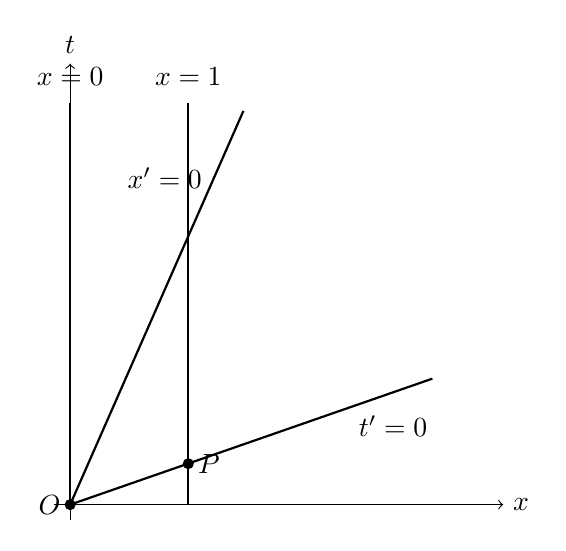
\begin{tikzpicture}[scale=1.0]
\draw[->] (-0.2,0) -- (5.5,0) node[right] {$x$};
\draw[->] (0,-0.2) -- (0,5.6) node[above] {$t$};
\draw[thick] (0,0) -- (0,5.1);
\draw[thick] (1.5,0) -- (1.5,5.1);
\draw[thick] (0,0) -- (2.2,5.0);
\draw[thick] (0,0) -- (4.6,1.6);
\fill (0,0) circle (2pt);
\fill (1.5,0.52) circle (2pt);
\node[left] at (0,0) {$O$};
\node[right] at (1.5,0.52) {$P$};
\node[above] at (0,5.2) {$x=0$};
\node[above] at (1.5,5.2) {$x=1$};
\node at (1.2,4.15) {$x'=0$};
\node at (4.1,1.0) {$t'=0$};
\end{tikzpicture}
\caption{A rod at rest in the unprimed frame. The moving observer measures its length along the tilted line \(t'=0\), not along a horizontal line of constant \(t\).}
\end{figure}

At the far endpoint \(P\), we know two things:
\begin{equation}
x=1,\qquad t'=0.
\end{equation}
From the Lorentz transformation,
\begin{equation}
t'=0 \quad \Longrightarrow \quad t=vx.
\end{equation}
Hence at \(P\),
\begin{equation}
t=v.
\end{equation}
In units with \(c=1\),
\begin{equation}
x'=\frac{x-vt}{\sqrt{1-v^2}},
\end{equation}
so
\begin{equation}
x'=\frac{1-v^2}{\sqrt{1-v^2}}=\sqrt{1-v^2}.
\end{equation}
Thus the moving observer measures the unit rod to have length
\begin{equation}
L'=\sqrt{1-v^2}.
\end{equation}
Restoring dimensions,
\begin{equation}
L=L_0\sqrt{1-v^2/c^2}=\frac{L_0}{\gamma}.
\end{equation}

Of course, in units with \(c=1\), the ``unit rod'' is whatever unit of length has been chosen to match the time unit; if time is measured in seconds, the natural length unit is a light-second. That bookkeeping detail does not affect the contraction factor.

The lecture is careful here: the rod does not merely \emph{look} shorter in some vague visual sense. The moving observer gives a precise operational definition using synchronized clocks and measuring rods, and with that definition the rod is shorter by the factor above.

\subsection{Time dilation}

Now take a clock carried by the moving observer. Its world line is
\begin{equation}
x'=0.
\end{equation}
Ask the following question: when the moving clock itself reads
\begin{equation}
t'=1,
\end{equation}
what time does the stationary frame assign to the corresponding event?

\begin{figure}
\centering
\begin{tikzpicture}[scale=1.0]
\draw[->] (-0.2,0) -- (4.3,0) node[right] {$x$};
\draw[->] (0,-0.2) -- (0,5.4) node[above] {$t$};
\draw[thick] (0,0) -- (0,4.8);
\draw[thick] (0,0) -- (1.7,4.2);
\draw[dashed] (1.7,4.2) -- (0,4.2);
\fill (0,0) circle (2pt);
\fill (1.7,4.2) circle (2pt);
\fill (0,4.2) circle (2pt);
\node[left] at (0,0) {$O$};
\node[right] at (1.7,4.2) {$R$};
\node[left] at (0,4.2) {$S$};
\node at (1.25,3.2) {$x'=0$};
\node[above] at (1.7,4.2) {$t'=1$};
\end{tikzpicture}
\caption{A moving clock. Proper time is measured along the slanted world line, while the stationary frame compares it with the coordinate time along the vertical axis.}
\end{figure}

Using the inverse transformation in units with \(c=1\),
\begin{equation}
t=\frac{t'+vx'}{\sqrt{1-v^2}},
\end{equation}
and setting \(x'=0\), \(t'=1\), we obtain
\begin{equation}
t=\frac{1}{\sqrt{1-v^2}}.
\end{equation}
So the stationary frame says that more time has elapsed than the moving clock itself records. In the usual notation,
\begin{equation}
\Delta t=\gamma\,\Delta t'.
\end{equation}
The moving clock runs slow.

This is already the seed of the twin paradox. If one twin goes away and comes back, then one world line is not a single inertial trajectory: it bends. The two twins are therefore not in symmetric situations. The traveling twin undergoes the turnaround, and that breaks the naive exchange symmetry.

\subsection{Question \& Answer}

Why is there no contradiction if each observer says the other meter stick is shorter?

Because the two observers are not talking about the same pair of spacetime events. The stationary observer measures length at one instant of stationary time. The moving observer measures length at one instant of moving time. Those are different slices of spacetime. Once length is defined correctly as an endpoint separation measured at equal time in the measuring frame, the two statements are perfectly compatible.

\section{The Invariant Interval, Proper Time, and the Strange Geometry of Spacetime}

At this point an audience member objects to the picture itself: how can the ``hypotenuse'' in spacetime come out shorter than the vertical side? Susskind agrees that this is exactly the right discomfort. It is the doorway to spacetime geometry.

He begins with an easier analogy. In the ordinary Euclidean plane, if two coordinate systems are related by a rotation, the coordinates of a point change, but the distance from the origin does not. In formulas,
\begin{equation}
x'^2+y'^2=x^2+y^2.
\end{equation}
That is the invariant of Euclidean rotations.

Now ask for the analogous invariant of Lorentz transformations. One might guess
\begin{equation}
t'^2+x'^2=t^2+x^2.
\end{equation}
The lecture tries this and rejects it. It is not true. Using the Lorentz transformation in units with \(c=1\),
\begin{align}
t'^2&=\frac{t^2+v^2x^2-2vtx}{1-v^2},\\
x'^2&=\frac{x^2+v^2t^2-2vtx}{1-v^2}.
\end{align}
Adding these does not give \(t^2+x^2\). The cross terms do not save us; the result is simply wrong.

But now subtract them:
\begin{align}
t'^2-x'^2
&=\frac{t^2+v^2x^2-2vtx}{1-v^2}
-\frac{x^2+v^2t^2-2vtx}{1-v^2}\\
&=\frac{(1-v^2)t^2-(1-v^2)x^2}{1-v^2}\\
&=t^2-x^2.
\end{align}
So the invariant quantity is
\begin{equation}
t'^2-x'^2=t^2-x^2.
\end{equation}
Restoring ordinary units, a standard form is
\begin{equation}
c^2t'^2-x'^2=c^2t^2-x^2.
\end{equation}

\begin{figure}
\centering
\begin{tikzpicture}[scale=1.0]
\draw[->] (-3.0,0) -- (3.8,0) node[right] {$x$};
\draw[->] (0,-0.2) -- (0,4.8) node[above] {$t$};
\draw[thick] (0,0) -- (3.4,3.4);
\draw[thick] (0,0) -- (-3.4,3.4);
\fill (1.1,3.5) circle (2pt);
\fill (2.8,1.4) circle (2pt);
\node[right] at (1.1,3.5) {timelike};
\node[right] at (2.8,1.4) {spacelike};
\node at (2.75,3.0) {$x=t$};
\node at (-2.55,3.0) {$x=-t$};
\end{tikzpicture}
\caption{The light rays \(x=\pm t\) divide spacetime into timelike and spacelike regions. The invariant interval changes sign across the light cone.}
\end{figure}

This is the quantity all observers agree on. Coordinates themselves are not invariant; they depend on the frame. The invariant interval does not.

Now suppose the two events lie on the world line of a moving clock. Then in the primed frame
\begin{equation}
x'=0,
\end{equation}
and the invariant reduces to
\begin{equation}
t'^2=t^2-x^2
\end{equation}
in units with \(c=1\). That quantity is the square of the proper time. In ordinary units,
\begin{equation}
\tau^2=t^2-\frac{x^2}{c^2}.
\end{equation}
Near the end of the lecture Susskind explicitly corrects the notation: proper time itself is the square root,
\begin{equation}
\tau=\sqrt{t^2-\frac{x^2}{c^2}}.
\end{equation}

For a light ray, the interval vanishes:
\begin{equation}
x^2-t^2=0
\qquad \Longleftrightarrow \qquad
x=\pm t
\end{equation}
in units with \(c=1\). So a lightlike separation has zero proper time. The lecture phrases this vividly: if a light beam could carry a clock, there would be no ticks between emission and absorption.

If
\begin{equation}
t^2-x^2>0,
\end{equation}
the separation is timelike, and the invariant is interpreted as proper time. If instead
\begin{equation}
x^2-t^2>0,
\end{equation}
the separation is spacelike, and one speaks of proper distance rather than proper time. In the spacelike case no physical object moving slower than light can connect the two events.

\subsection{Question \& Answer}

How can the spacetime hypotenuse be shorter than the vertical side, and when does the invariant become proper time rather than proper distance?

The first answer is simply that spacetime geometry is not Euclidean geometry. The invariant involves a difference of squares, not a sum. That minus sign makes the quantity associated with a slanted timelike world line smaller than the pure time separation along the vertical axis. The ``hypotenuse'' is shorter because the geometry itself is different.

The second answer is causal. If the two events can be connected by the world line of a physical clock, the separation is timelike and the invariant gives proper time. If no subluminal trajectory can connect them, the separation is spacelike and the corresponding invariant is interpreted as proper distance. If the separation is null, a light ray connects the events and the proper time is zero.

The lecture closes with a short historical reflection. Einstein's guiding clue was not merely an experimental correction to Newtonian mechanics, but the recognition that Maxwell's equations point to a different symmetry of space and time. Lorentz had related formulas, and he tied them to motion through the ether. Einstein made the stronger move: he treated the symmetry itself as a principle.

\section{Summary}

Special relativity begins here not with a miraculous formula but with a contradiction. If we keep the Galilean transformation, light does not have the same speed in every inertial frame. The way out is not to abandon the light postulate, but to abandon universal simultaneity. Once synchronization is defined operationally with light signals, the moving notion of simultaneity can be drawn geometrically, and from that geometry one derives the Lorentz transformation. The immediate consequences are length contraction and time dilation, and the deeper payoff is the invariant interval
\begin{equation}
t'^2-x'^2=t^2-x^2,
\end{equation}
or in ordinary units \(c^2t'^2-x'^2=c^2t^2-x^2\). That invariant is the real structural object of the chapter. Coordinates depend on the observer; the interval does not. In the next lecture, this geometry will be used to understand the motion of particles.